\documentclass{article}

\usepackage{graphicx}
\usepackage{subcaption}
\usepackage{geometry}
\usepackage{hyperref}
\usepackage[numbered,framed]{matlab-prettifier}
\usepackage{filecontents}
\usepackage{float}
\usepackage{wrapfig}

\usepackage{listings}
\usepackage{color} %red, green, blue, yellow, cyan, magenta, black, white
\definecolor{mygreen}{RGB}{28,172,0} % color values Red, Green, Blue
\definecolor{mylilas}{RGB}{170,55,241}

%https://it.sharelatex.com/learn/Positioning_images_and_tables

% =================== End preamble =================

\begin{document}

\lstset{language=Matlab,%
    %basicstyle=\color{red},
    breaklines=true,%
    morekeywords={matlab2tikz},
    keywordstyle=\color{blue},%
    morekeywords=[2]{1}, keywordstyle=[2]{\color{black}},
    identifierstyle=\color{black},%
    stringstyle=\color{mylilas},
    commentstyle=\color{mygreen},%
    showstringspaces=false,%without this there will be a symbol in the places where there is a space
    numbers=left,%
    numberstyle={\tiny \color{black}},% size of the numbers
    numbersep=9pt, % this defines how far the numbers are from the text
    emph=[1]{for,end,break},emphstyle=[1]\color{red}, %some words to emphasise
    %emph=[2]{word1,word2}, emphstyle=[2]{style},    
}

% ================== Title =========================
\begin{titlepage}
\newcommand{\HRule}{\rule{\linewidth}{0.1 mm}}
\center
\textsc{\Large Politecnico di Torino}\\[0.3cm]
\HRule\\[0.5cm]
{\huge \bfseries ICT for health}\\[0.05cm]
\HRule\\[0.1cm]
\vspace{1cm}
\center {
\includegraphics[scale=0.5]{pictures/logo.jpg}}\\[2cm]
\Large Academic Year 2016/2017\\[3cm]
\iffalse\begin{multicols}{2}
\columnbreak
\end{multicols}\fi
\begin{minipage}{1\textwidth}
\vspace{3cm}
\textbf{\underline{Professors:}}
\hfill
\textbf{\underline{Author:}} \\
Monica Visintin
\hfill
Gaetano Moceri\\
Guido Pagana
\end{minipage}
\end{titlepage}	
% ================== End title ========================

\pagenumbering{gobble}
\newpage
\tableofcontents
\pagenumbering{roman}
\newpage
\pagenumbering{arabic}

\section{Introduction}
The purpose of this report is to explain how laboratory activities within the "ICT for Health" subject have been faced. Each chapter is related to a single topic. In order to allow readability, within each section there will be just an introduction and the explaination of what it was done by introducing some significant code lines and graphs. The whole set of codes and plots is placed at the end of each descriptive section. 

\section{Linear regression - PCR - Neural Networks}
\subsection{Introduction}
Linear regression and Principal Component Regression (PCR) are machine learning techniques which allow the prevision of some future values starting from a set of known samples. This machine learning approach is called supervised learning and performes predictive analysis. PCR is a more complex technique: regression is carried out after a data manipulation that leads to the selection of a subset of the initial dataset (Principal Component Analysis). Neural networks will be treated in the following paragraphs.
The dataset comes from UCI Machine Learning repository (\href{https://archive.ics.uci.edu/ml/datasets/Parkinsons+Telemonitoring}{link dataset}).\\

The aim of the laboratory is performing linear regression on feature 5 and feature 7 of the initial dataset, which are respectively clinician's motor linearly interpolated UPDRS score and a measured voice parameter (jitter in percentage). The expected result is that measured feature will regress better with respect to the interpolated one.

\subparagraph{Data cleaning and normalization} 
Is the very first operation to be done on the raw data. It is a sort of filtering unreliable and wrong or missing data and guarantees data correctness. The "dataLoading" function aims to perform this task.\\

Then, it is convenient to normalize data measured in different scales in order to make featuers coherent with each other. From a pratical point of view, normalizing a dataset means remove averages and make variances equal to one.\\
Click \ref{lst: Data cleaning function} for the code.

\subsection{Linear regression}
From the normalized dataset, it is possible to apply machine learning algorithms. \\

Linear regression in particular, models the relationship between one or more scalar dependent variables, called regressors, and a dependent variable, called regressand. The focus is on finding a linear function that links the regressors and the regressand. Linear function consists in finding some weights which link the dependent variable with the independent ones. Parameters of this linear function are estimated starting from data and different methodologies can be used.\\

\subparagraph{Minimum Square Error}
This method calculates the best-fitting line for the observed data by minimizing the sum of the squares of the vertical deviations from each data point to the line: if a point lies on the fitted line exactly, then its vertical deviation is 0, so error is null.
Minimum square error (MSE) is an estimation method which minimizes the square error of the observed values and the fitted ones. From a conceptual point of view, the error function is derived  in order to find the set of parameters which minize it.
The graphs show the output of the MSE algorithm. Figure \ref{fig:MSE_F5} deals with the interpolated feature. While figure \ref{fig:MSE_F7} shows the result for feature 7. Click \ref{lst: MSE coefficients} for the code.

\begin{figure}[H]
	\centering
	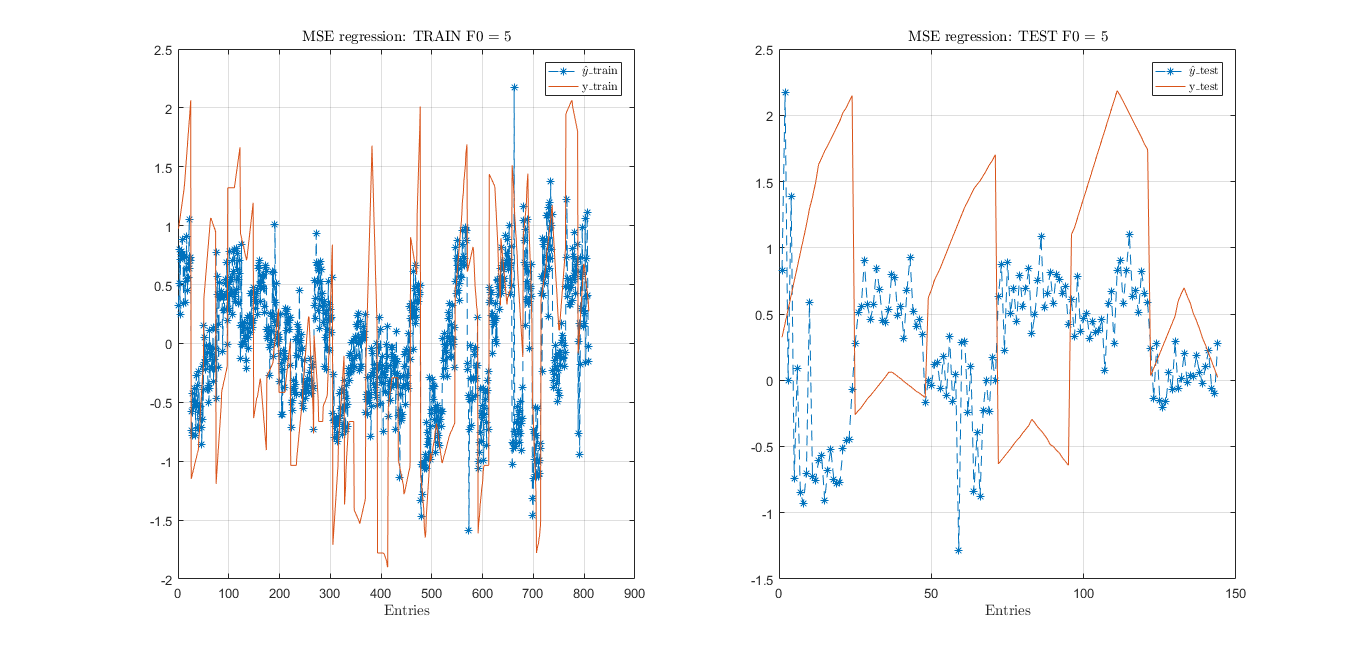
\includegraphics[scale=0.3]{pictures/MSE_F5_2.png}
	\caption{MSE estimation plots for feature 5}\label{fig:MSE_F5}
\end{figure}

\begin{figure}[H]
	\centering
	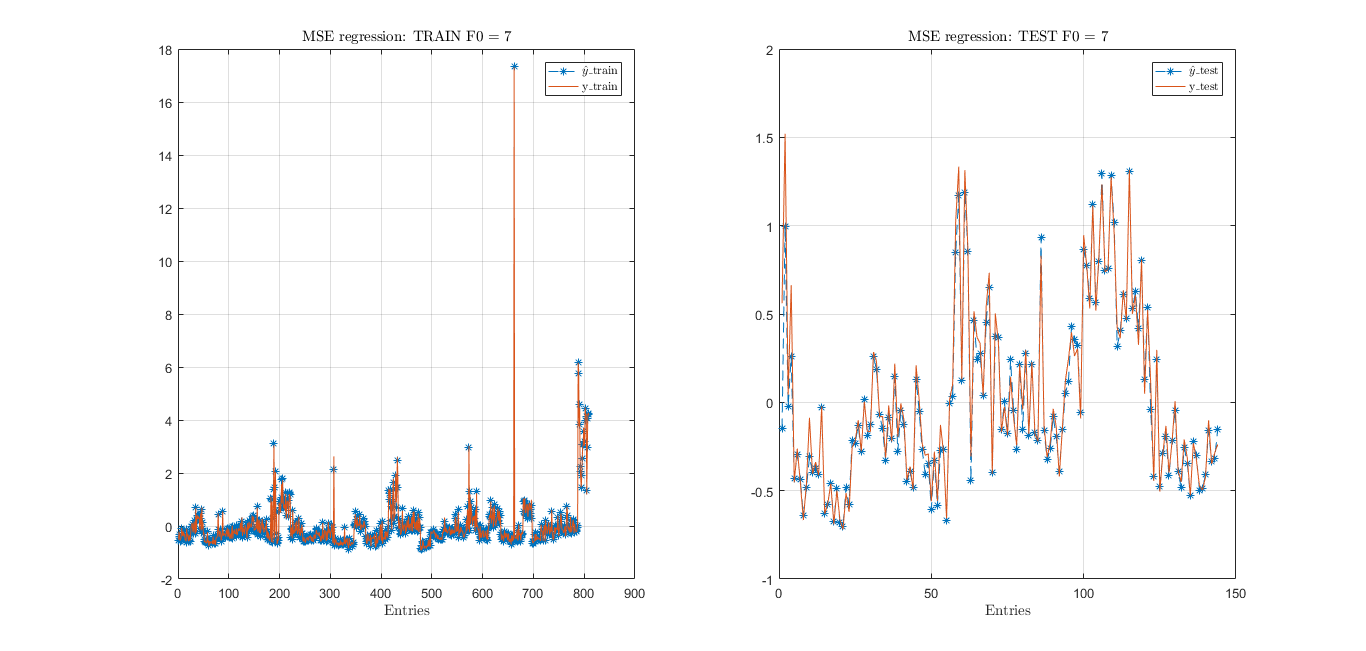
\includegraphics[scale=0.3]{pictures/MSE_F7_2.png}
	\caption{MSE estimation plots for feature 7}\label{fig:MSE_F7}
\end{figure}

As it was expected, feature 5 is very bad fitted because it deals with the physician judgment: it is uncorrelated with the other features and is difficoult to be predicted. The errors in both train and test phase show a very high variance and regression is (see below for the other graphs). On the other side, feature 7 is related to voice characteristics: in this case prediction is very accurated and  regression is much more linear than before. 

\subparagraph{Gradient Algorithm}
Since MSE technique requires the train matrix inversion, which could require a lot of computational and time resources in the case of a lot of matrix entries, an iterative solution is suited. In particular, gradient algorithm (GA) allows to find local minimum of a function from an initial guess of the coefficients. Each iteration, a "jump" toward the minimum is performed: the direction of the jump comes from the gradient (negative), while the length is given by a learning coefficient greater than zero. Learning coefficient should be properly choosen: if it is too small there could be a lot of iterations before reaching a good solution. If it is too large, jumps may not reach an optimal solution and remaining in a loop around the local minimum.
A stopping condition should block the iterations when the distance from the previous solution is smaller than a threshold. 
GA result seems very similar to the MSE one, but computational time is almost 20 times larger from the learning coefficient and threshold choosen values. Click \ref{lst: GA coefficients function} for the code.

\subparagraph{Steepest Descent}
Steepest descent (SD) is an iterative algorithm very similar to the gradient algorithm, discussed previously. The difference is that here the step size is adaptive: learning coefficient is updated each iteration. While the same threshold and the same stopping condition used in gradient algorithm are applied in steepest descent. Click \ref{lst: SD coefficients function} for the code.

\subparagraph{Conclusions}
From the graphs generated, (\ref{fig:GA_F5_FINAL}, \ref{fig:GA_F7_FINAL}, \ref{fig:MSE_F5_FINAL}, \ref{fig:MSE_F7_FINAL}, \ref{fig:MSE_F7}, \ref{fig:SD_F5_FINAL}, \ref{fig:SD_F7_FINAL}) the results of the three algorithm discussed are very similar each other, in terms of errors estimation. The main difference is the computational time: with the configurated parameters, MSE and SD have a comparable execution time, while GA execution time is 10-15 time higher. For both features, it has also been computated the iterations number for the iterative algorithms: SD has about 1000 iterations, while GA performs 100 times the number of SD iterations, maybe due to the fact that SD adapts the step size by updating the learning coefficient. 

\subsection{Principal Component Regression}
Principal component regression (PCR) is a kind of regression performed from a simplified version of the dataset. The "simplification" process is actuated by principal component analysis (PCA) where initial features are projected in a new space through an orthonormal basis computed from covariance matrix of the initial train dataset. Then, new features are statistically indepentent. Click \ref{lst: PCR coefficients function} for the code.

\begin{wrapfigure}{l}{0.5\textwidth}
	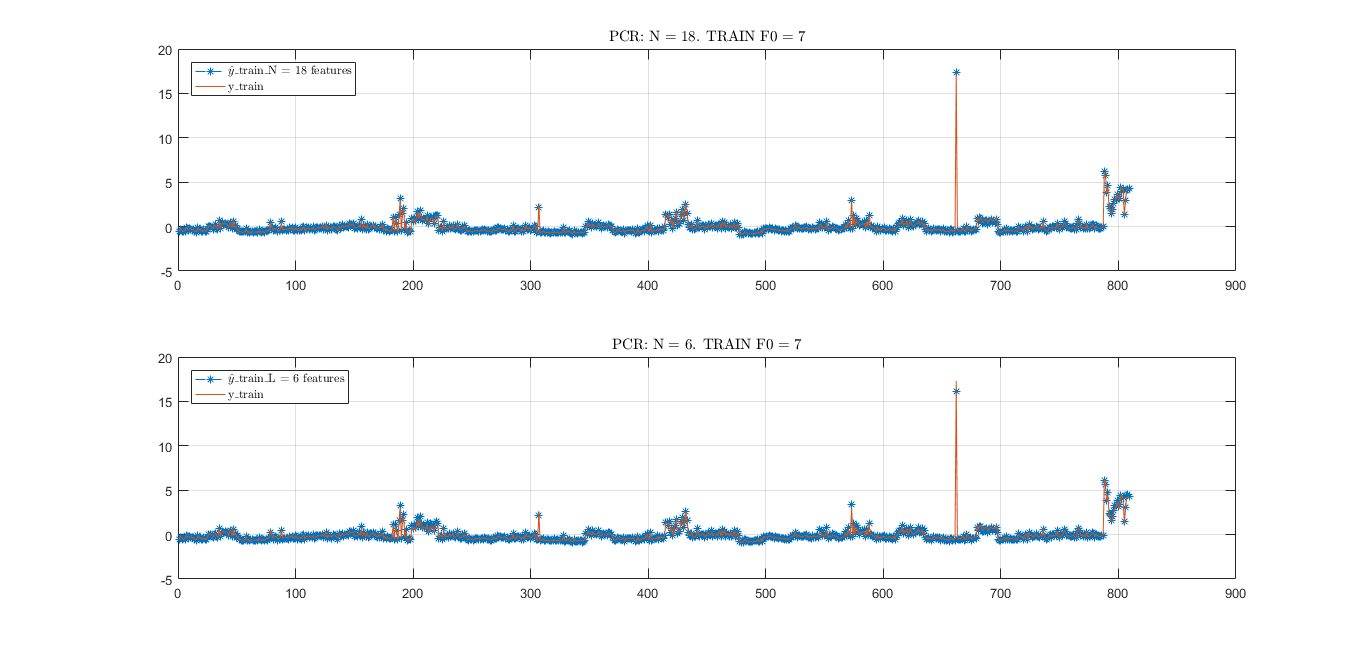
\includegraphics[width=1\linewidth]{pictures/PCR.png} 
	\caption{PCR estimation for both features}
	\label{fig:PCR}
\end{wrapfigure}

From the basis, eigenvectors with the corresponding highest eigenvalues are more "important" and correspond to the variables with the highest variance: eigenvectors with lower eigenvalues have to be descarded because the corresponding features are less meaningful: pratically, it is possible to discard them in order to simplify the dataset. In this case, the 90\% of the eigenvalues total sum is considered, corresponding to "L" features.
Performances are still similar to the other algorithms described (MSE and SD), but now the set of coefficients is more regular and from figure \ref{fig:PCR} is possible to see how this method underestimate the big outlier, in the inner graph. \\

For very complex dataset, PCA is fundamental because it allows feature extraction and consequentely data simplification. Another advantage of PCR is that it is very robust against outliers, as told before, but on the other side, since a part of data is going to be "thrown away", performance, in terms of error are worse with respect to the other algorithms. \\
Below, you find all scripts and plots for the regression task.

\lstinputlisting[caption = {UPDRS Analysis - Main}]{scripts/UPDRSAnalysis_FINALVERSION.m}\label{lst: UPDRS analysis - Main}
\lstinputlisting[caption = {Data cleaning function}]{scripts/dataLoading.m}\label{lst: Data cleaning function}
\lstinputlisting[caption = {Data normalization function}]{scripts/matNorm.m}\label{lst: Data normalization function}
\lstinputlisting[caption = {MSE coefficients function}]{scripts/MSECoefficients.m}\label{lst: MSE coefficients}
\lstinputlisting[caption = {Plot function}]{scripts/estimPlot.m}\label{lst: Plot function}

\begin{figure}[H]
	\centering
	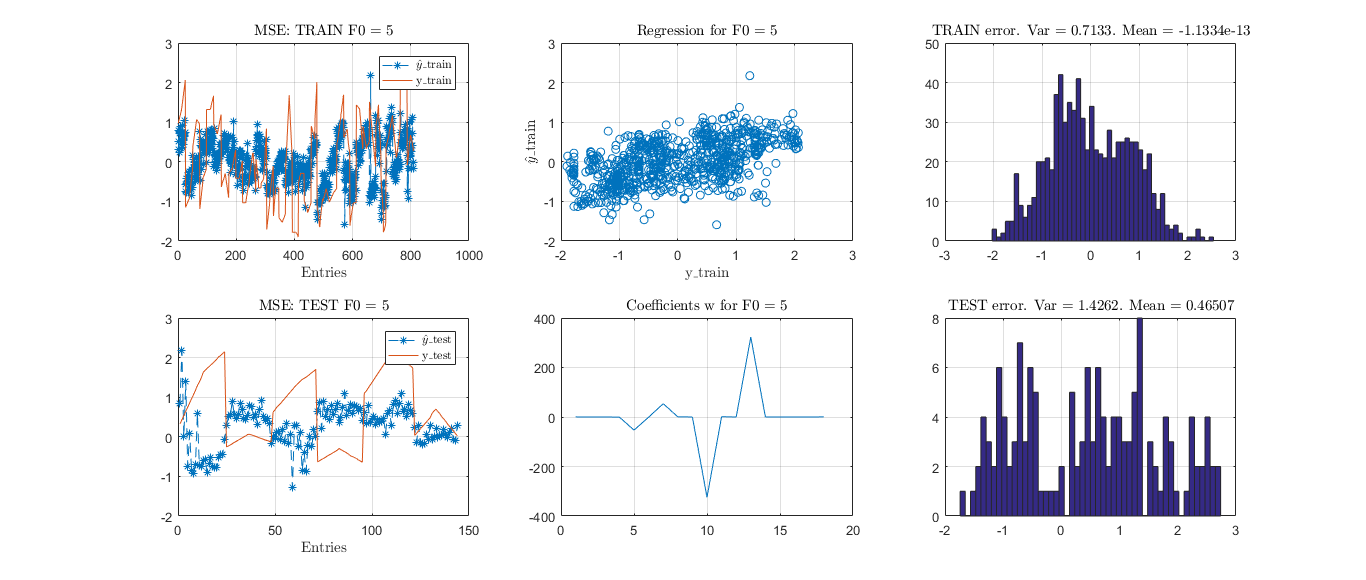
\includegraphics[width=0.9\textwidth]{pictures/MSE_F5_FINAL.png}
	\caption{MSE estimation plots for feature 5}\label{fig:MSE_F5_FINAL}
\end{figure}

\begin{figure}[H]
	\centering
	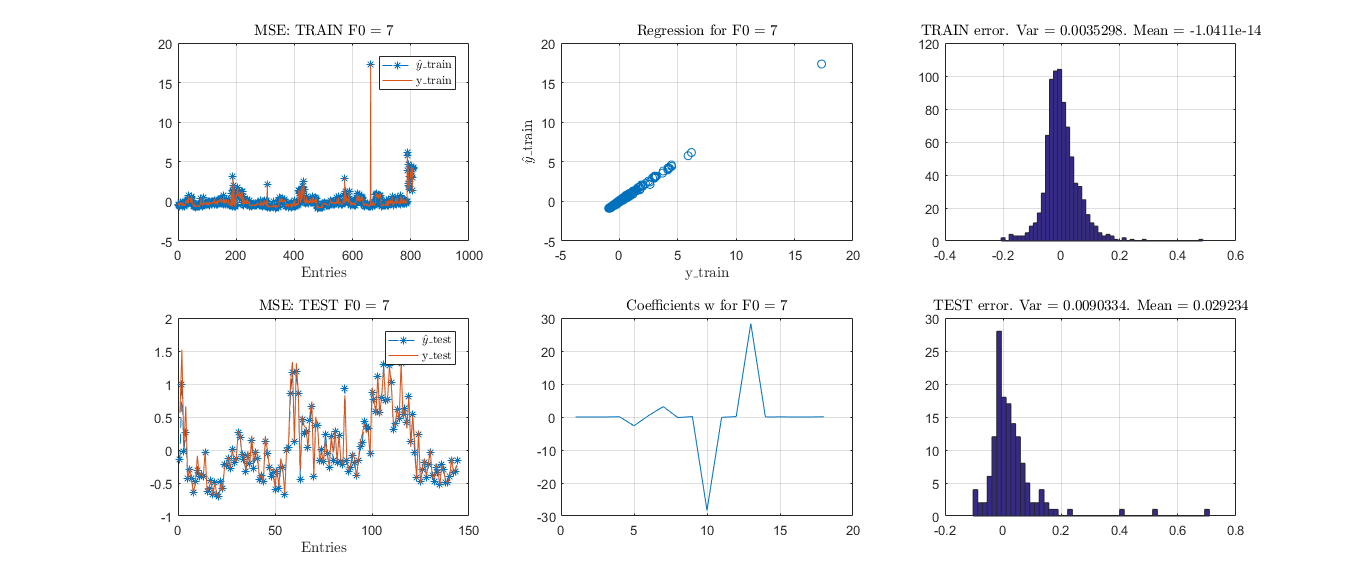
\includegraphics[width=0.9\textwidth]{pictures/MSE_F7_FINAL.png}
	\caption{MSE estimation plots for feature 7}\label{fig:MSE_F7_FINAL}
\end{figure}

\lstinputlisting[caption = {GA coefficients function}]{scripts/GACoefficients.m}\label{lst: GA coefficients function}

\begin{figure}[H]
	\centering
	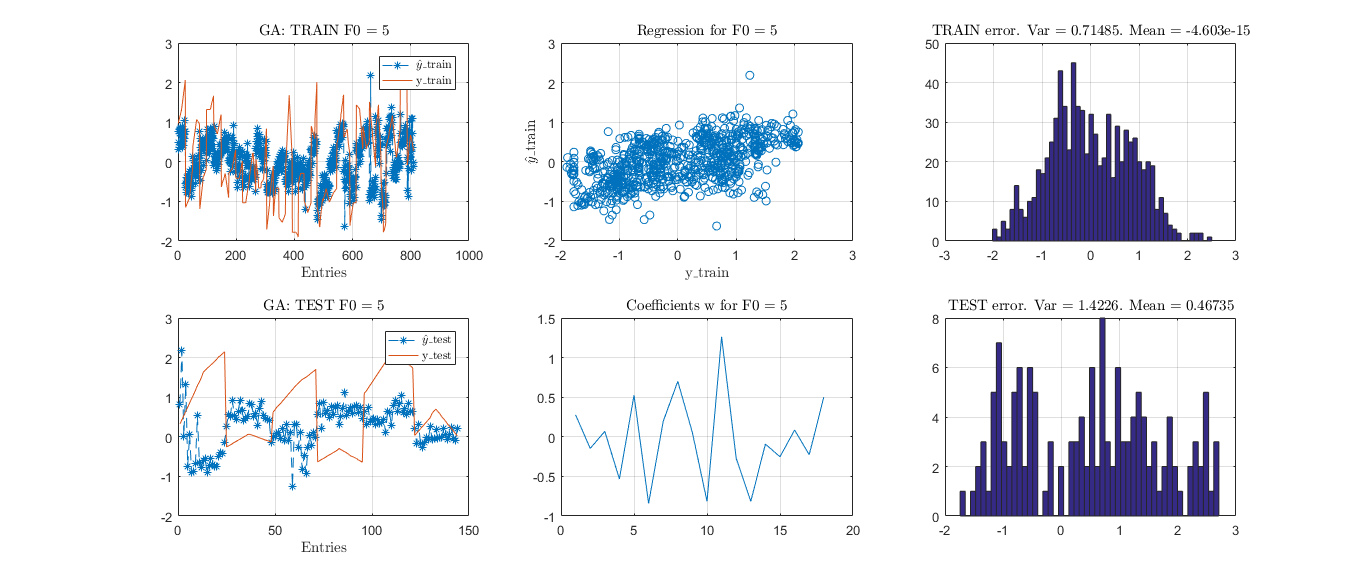
\includegraphics[width=0.9\textwidth]{pictures/GA_F5_FINAL.png}
	\caption{GA estimation plots for feature 5}\label{fig:GA_F5_FINAL}
\end{figure}

\begin{figure}[H]
	\centering
	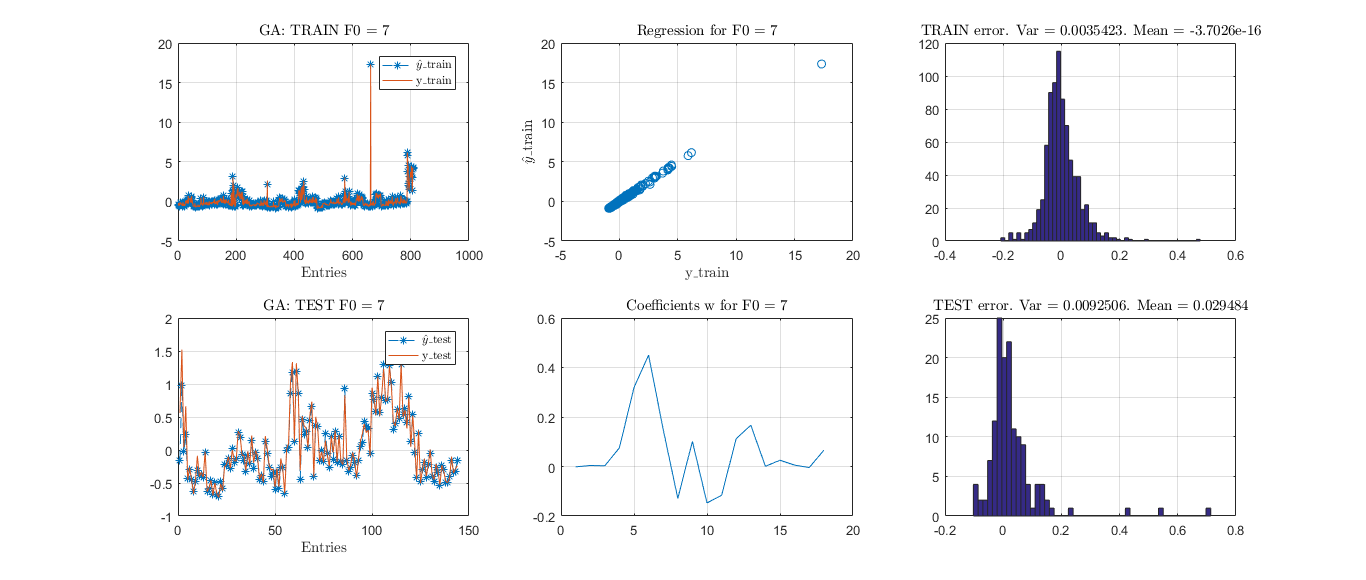
\includegraphics[width=0.9\textwidth]{pictures/GA_F7_FINAL.png}
	\caption{GA estimation plots for feature 7}\label{fig:GA_F7_FINAL}
\end{figure}

\lstinputlisting[caption = {SD coefficients function}]{scripts/SDCoefficients.m}\label{lst: SD coefficients function}

\begin{figure}[H]
	\centering
	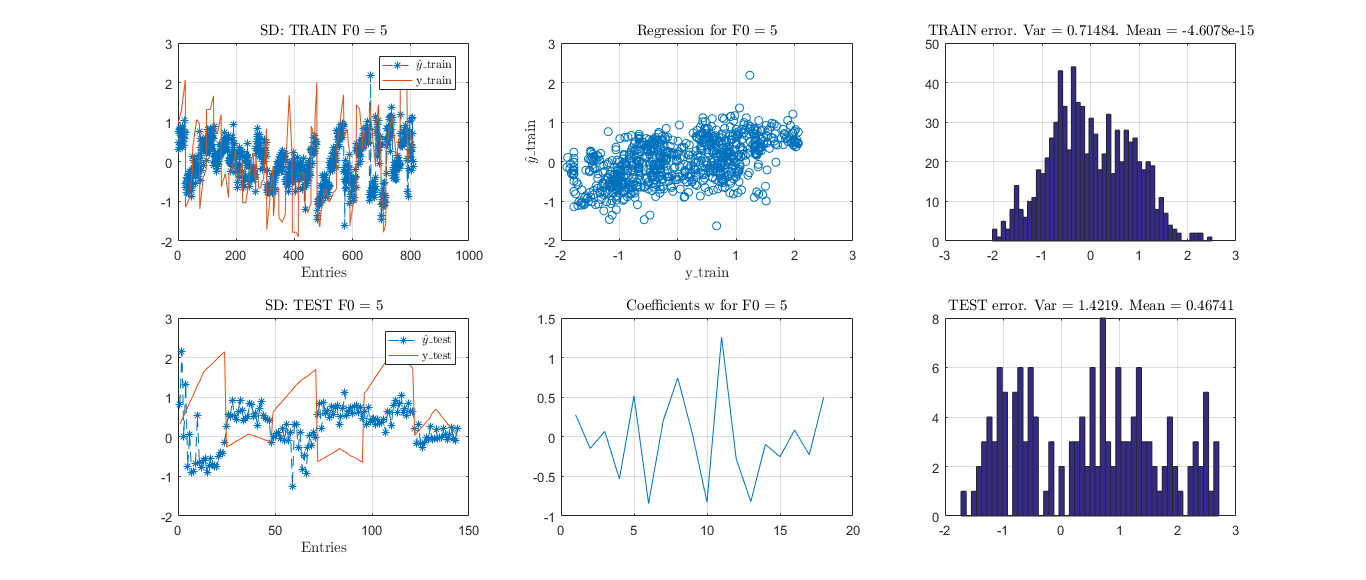
\includegraphics[width=0.9\textwidth]{pictures/SD_F5_FINAL.png}
	\caption{SD estimation plots for feature 5}\label{fig:SD_F5_FINAL}
\end{figure}

\begin{figure}[H]
	\centering
	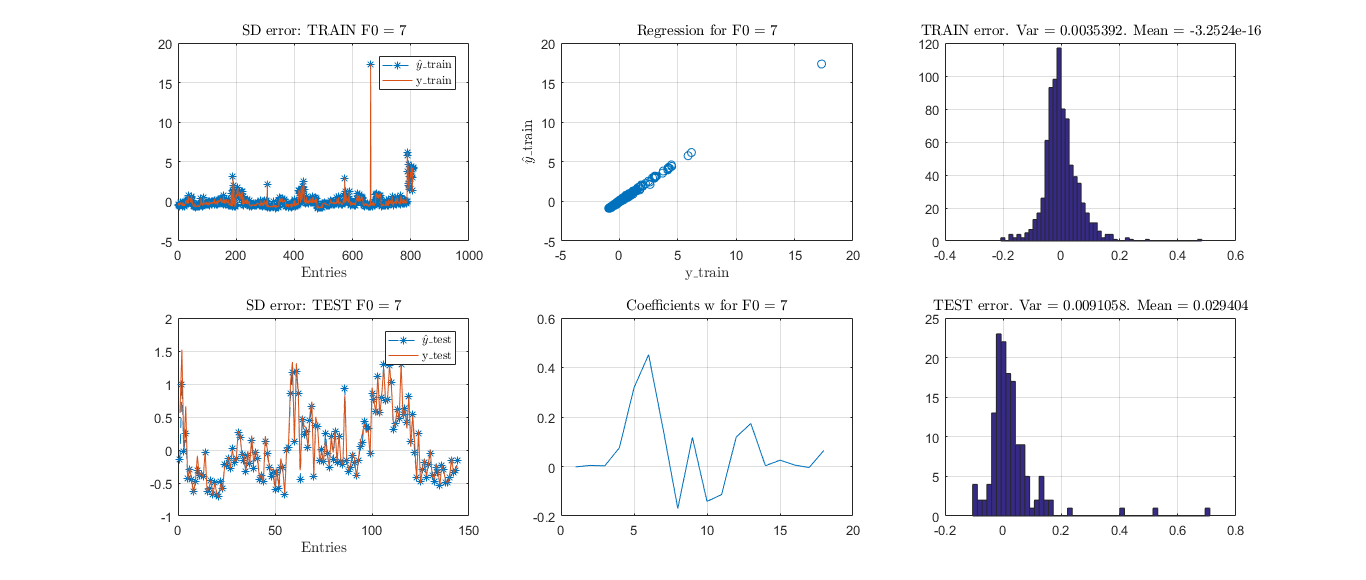
\includegraphics[width=0.9\textwidth]{pictures/SD_F7_FINAL.png}
	\caption{SD estimation plots for feature 7}\label{fig:SD_F7_FINAL}
\end{figure}

\lstinputlisting[caption = {PCR coefficients function}]{scripts/PCRCoefficients.m}\label{lst: PCR coefficients function}
\lstinputlisting[caption = {PCR plot function}]{scripts/estimPlotPCR.m}\label{lst: PCR plot function}

\begin{figure}[H]
	\centering
	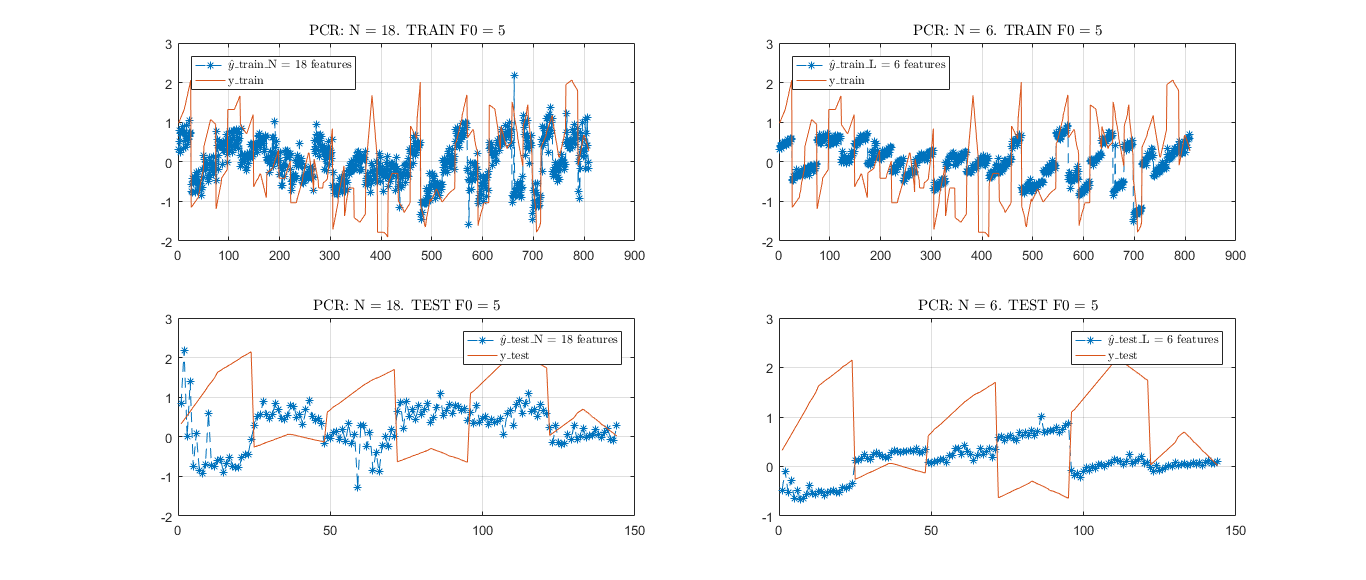
\includegraphics[width=0.9\textwidth]{pictures/PCR_F5_FINAL.png}
	\caption{PCR estimation plots for feature 5}\label{fig:PCR_F5_FINAL}
\end{figure}

\begin{figure}[H]
	\centering
	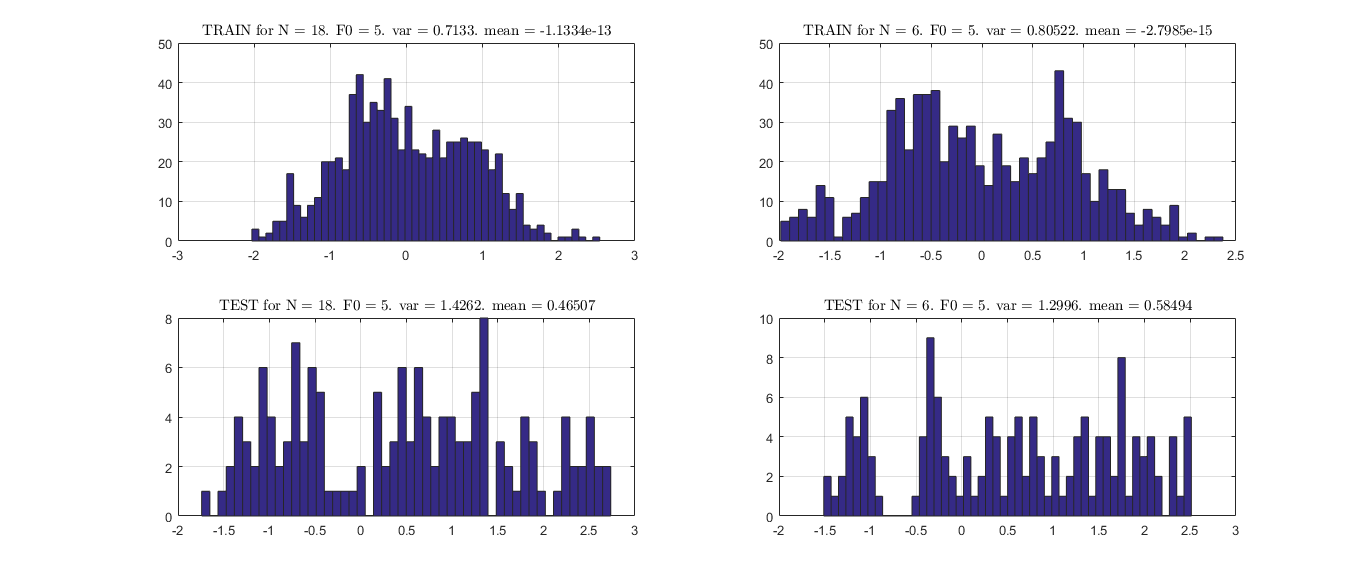
\includegraphics[width=0.9\textwidth]{pictures/PCR_F5_ERRORS.png}
	\caption{PCR error plots for feature 5}\label{fig:PCR_F5_ERRORS}
\end{figure}

\begin{figure}[H]
	\centering
	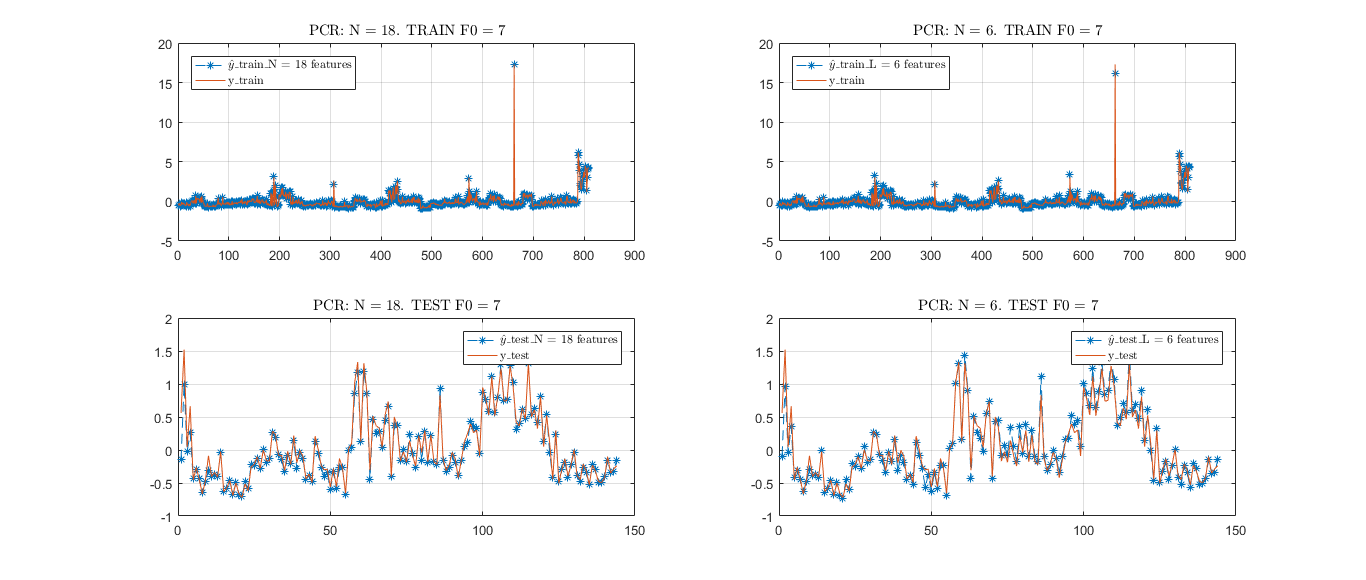
\includegraphics[width=0.9\textwidth]{pictures/PCR_F7_FINAL.png}
	\caption{PCR estimation plots for feature 7}\label{fig:PCR_F7_FINAL}
\end{figure}

\begin{figure}[H]
	\centering
	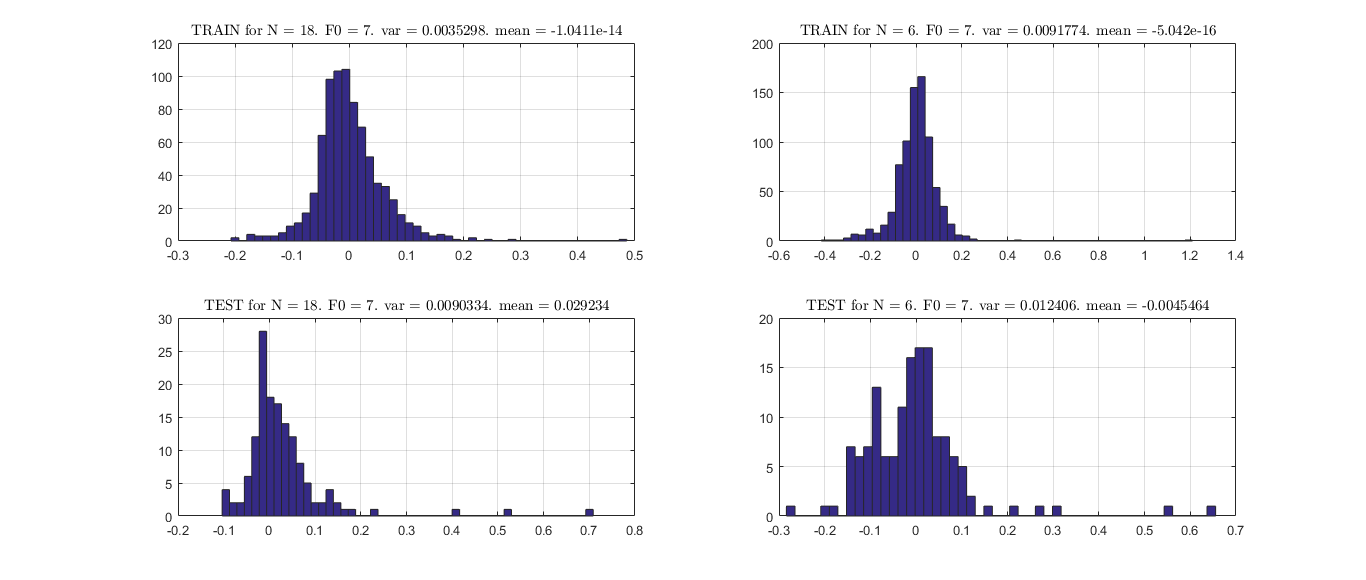
\includegraphics[width=0.9\textwidth]{pictures/PCR_F7_ERRORS.png}
	\caption{PCR error plots for feature 7}\label{fig:PCR_F7_ERRORS}
\end{figure}

\begin{figure}[H]
	\centering
	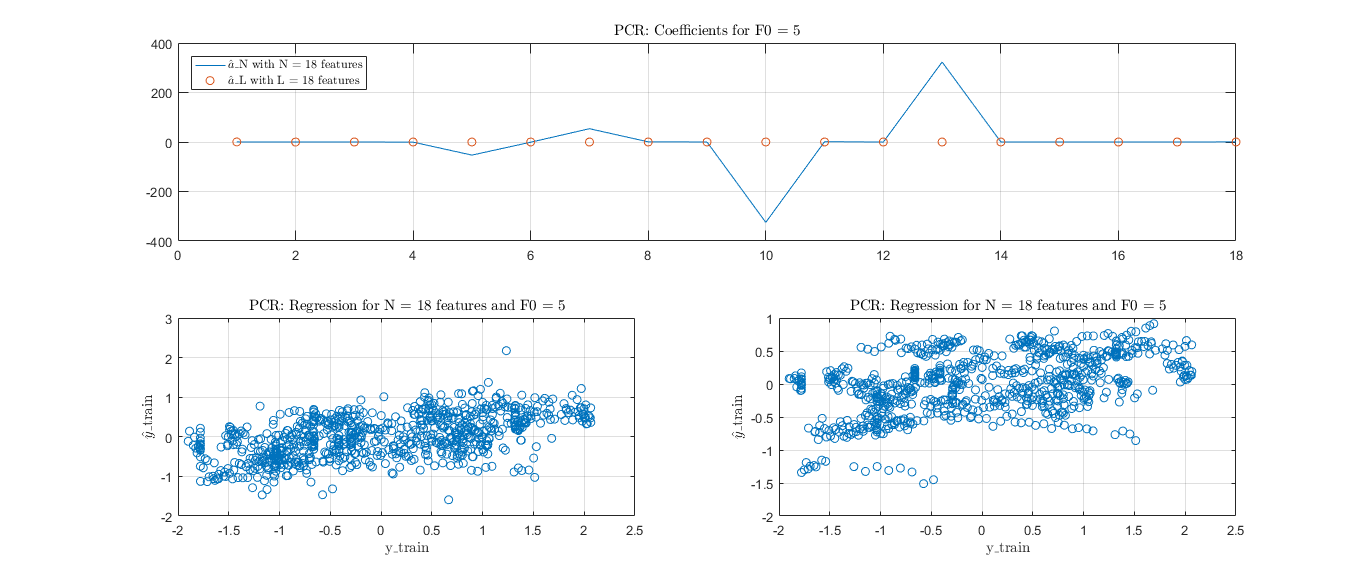
\includegraphics[width=0.9\textwidth]{pictures/PCR_F5_REGRESSION.png}
	\caption{PCR regression plots for feature 5}\label{fig:PCR_F5_REGRESSION}
\end{figure}

\begin{figure}[H]
	\centering
	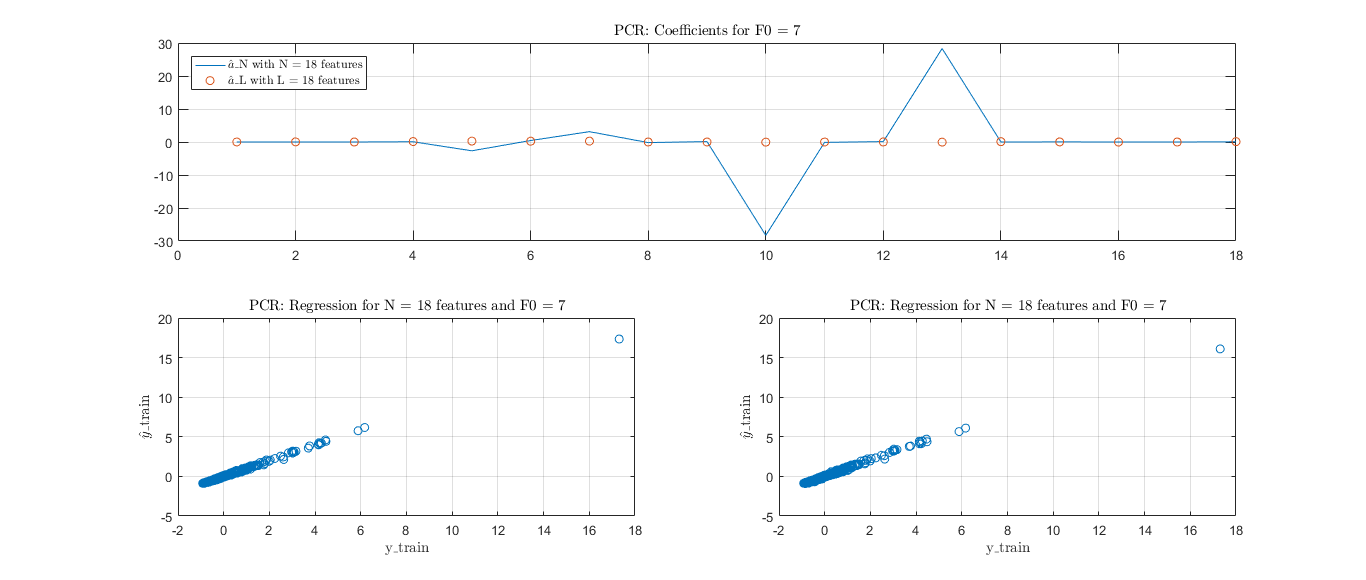
\includegraphics[width=0.9\textwidth]{pictures/PCR_F7_REGRESSION.png}
	\caption{PCR regression plots for feature 7}\label{fig:PCR_F7_REGRESSION}
\end{figure}

\newpage
\subsection{Neural networks - Introduction}
Regression task was also performed by using neural networks. For this exercise it has been used Python programming language with Google Tensorflow library. Initial dataset is already normalized. Typically, neural networks use a gradient algorithm approach by applying backpropagation method: Tensorflow allows to do it very easily. Tensorflow approach is divided in two parts: building the neural network "hardware" and runing the computational graph.\\
In order to compare performances with MATLAB ones, the parameters are the same. Check \ref{lst: ANN regression} for the whole code. A menu was implemented in order to allow the user to choose if to perform a no hidden layers regression or a two hidden layers regression. Code is shown here \ref{lst: ANN regression}.

\subsubsection{No hidden layers regression}
In no hidden layers case, as it was expected, feature 5 is still very badly fitted with a huge error variance, which is very similar to the MATLAB case shonw in \ref{fig:GA_F5_FINAL}. While feature 7, as it was expected again, seems to be very well estimated on both train an test phase. Error histogram is quite similar to the MATLAB gradient algorithm analysis in \ref{fig:GA_F7_FINAL}. It is reasonable because the learning coefficient is exactly the same, and the iterations number is of the same order of magnitude. 

\subsubsection{Two hidden layers regression}
In this case, neural network implements two hidden layers. The first one has 17 nodes and the second one 10. Here, training performances seems very good in feature 5  training context, as it is shown in the figure \ref{fig:regrF52HL} beside: regression is quite good and errors histogram presents a very low variance. But when the model is tested, result gets worse than the "no hidden layers" case. It could be a clear example of overfitting: it means that the model learns perfectly the train dataset features, but it is not able to predict the new observations. In this case, the model found is not usable. This happens when, for example, parameters number is big with respect to the observations or when the training runs for too much time. Cross-validation may be a very usefull method to prevent overfitting.

\begin{figure}[h]
 
\begin{subfigure}{0.5\textwidth}
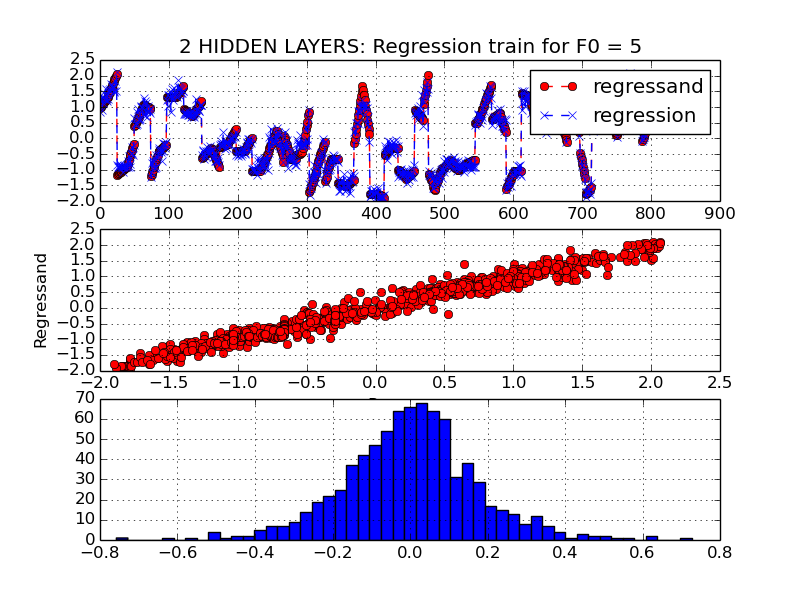
\includegraphics[width=0.9\linewidth, height=5cm]{pictures/regrF52HL.png} 
\caption{ANN training for F 5}
\label{fig:regrF52HL}
\end{subfigure}
\begin{subfigure}{0.5\textwidth}
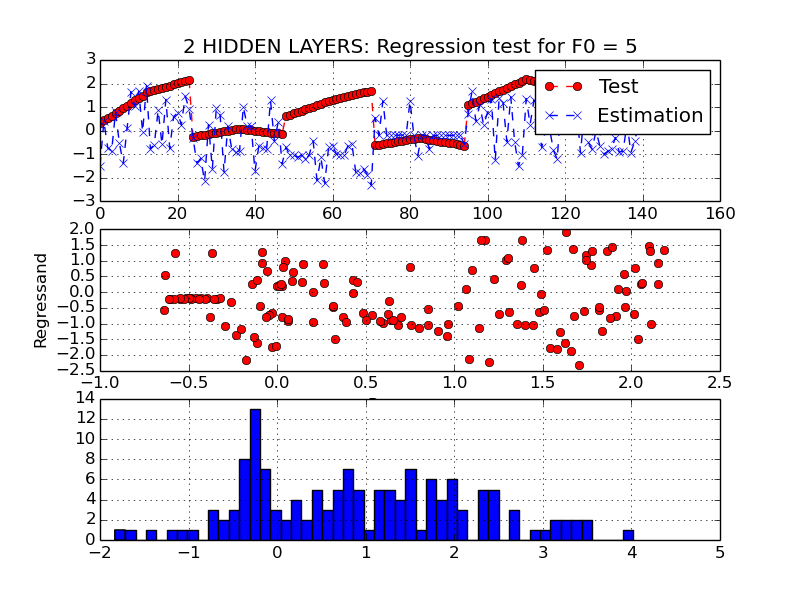
\includegraphics[width=0.9\linewidth, height=5cm]{pictures/regrF52HL_TEST.png}
\caption{ANN testing for F 5}
\label{fig:regrF52HL_TEST}
\end{subfigure}
 
\caption{Regression plots for F 5 with 2 hidden layers}
\label{fig:regrF52HL_PLOTS}
\end{figure}

The same discussion is valid for feature 7: the training phase is very good and the error histogram shows that error is enormously small (Fig.\ref{fig:regrF57HL_PLOTS}). But when the model is tested, it gets worse than the "no hidden layers" case because of overfitting, again. In general, introducing some new hidden layers in neural networks, gets worse results. For what concern the neurons number, there is an empirical rule saying that "the optimal size of the hidden layer is usually between the size of the input and size of the output layers".

\begin{figure}[h]
 
\begin{subfigure}{0.5\textwidth}
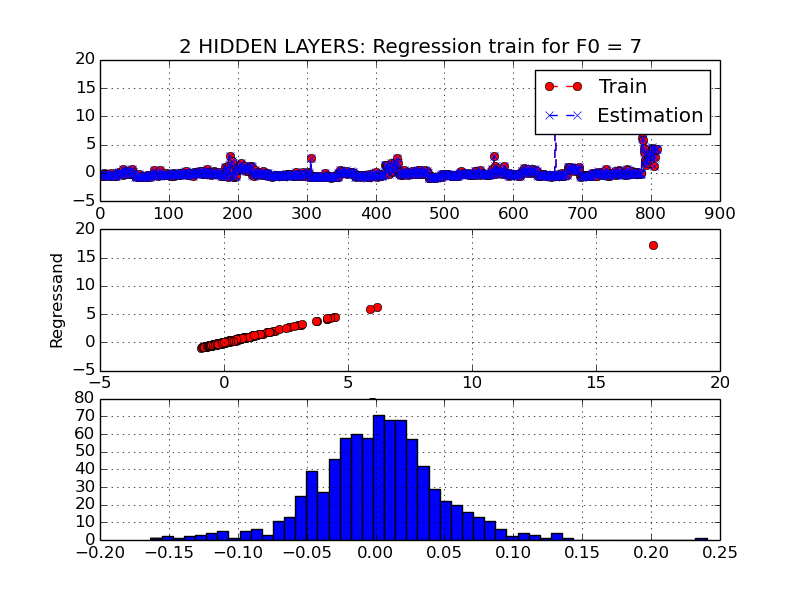
\includegraphics[width=0.9\linewidth, height=5cm]{pictures/regrF72HL.png} 
\caption{ANN training for F 7}
\label{fig:regrF57HL}
\end{subfigure}
\begin{subfigure}{0.5\textwidth}
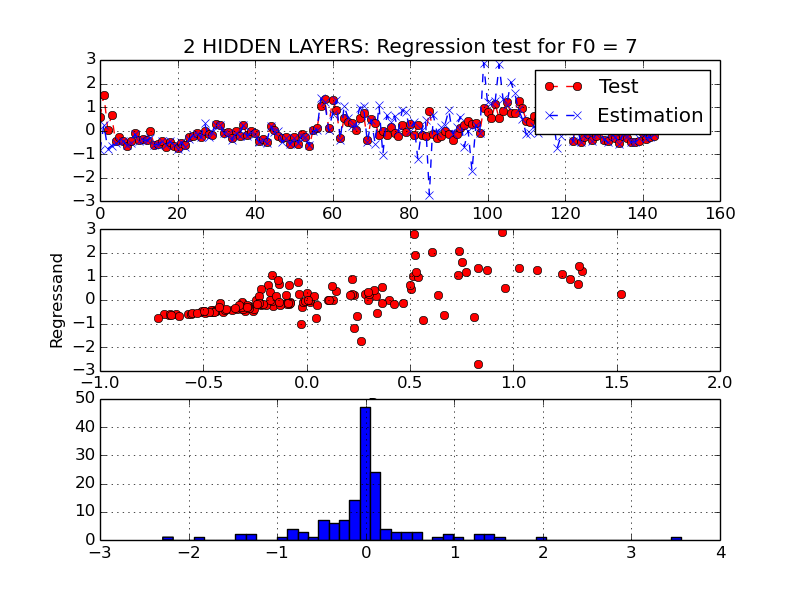
\includegraphics[width=0.9\linewidth, height=5cm]{pictures/regrF72HL_TEST.png}
\caption{ANN testing for F 7}
\label{fig:regrF57HL_TEST}
\end{subfigure}
 
\caption{Regression plots for F 7 with 2 hidden layers}
\label{fig:regrF57HL_PLOTS}
\end{figure}


\lstinputlisting[caption = {Neural network regression}]{scripts/Exercise6.py}\label{lst: ANN regression}

\begin{figure}[H]
	\centering
	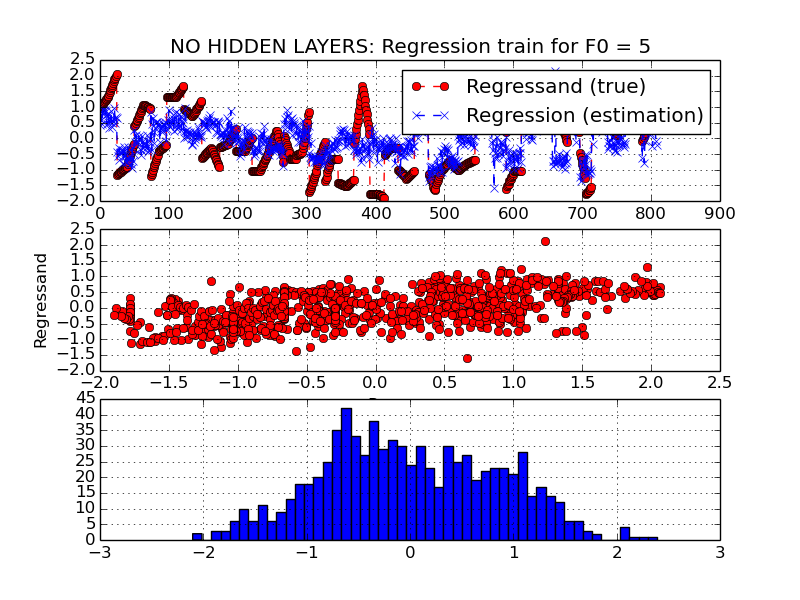
\includegraphics[width=0.9\textwidth]{pictures/regrF5NOHL.png}
	\caption{ANN regression F = 5 with no HL}\label{fig:regrF5NOHL}
\end{figure}


\newpage
\section{Classification}
\subsection{Introduction}
Classification problems focus on identifying to which set of categories a new observation belongs to. As linear regression, classification algorithms are considered instances of supervised learning. From a conceptual point of view, classification techniques try to recognize patterns and regularities in train dataset labeled with true classes. Each class is conceptually summarized by a representative value, called centroid. In general, a new observation belongs to the class at the minimum distance with respect to the others.\\

Dataset is from UCI Machine learning repository (\href{http://archive.ics.uci.edu/ml/datasets/Arrhythmia}{link dataset}). The aim of this exercise is performing 2 classification algorithms and testing their performances. Dataset contains 279 attributes related to ECG track. Last column is contains patient's scores, going from 1 to 16, where 1 suggests healthy patients, from 2 to 15 it indicates different levels of arrythmia, while 16 refers to an unclassified status of the sickness. \\
The code is placed at the end of clustering section(\ref{lst: Arrythmia analysis - Main}) because of an easier results readability.

\subparagraph{Data cleaning and normalization}
Since dataset contains some missing or wrong data, a cleaning process is the first thing to do, made by deleting empy features (columns). Next, as it has been said above, normalization must be done in order to get attributes coherent with each other through removing the mean and setting variance to one. 

\subsection{Binary classification}
The first task requires binary classification. Considered classes are 1, which is related to healty patients, and 2, that gathers all sick patients and unclassified ones. From the knowledge of the classes, it is possible to choose the decision function that maps the observed values to the regions. There are several kinds of classification algorithms, and it is important keeping in mind that different decision criteria give rise to different decision regions and, of course, different results.

\subsubsection{Minimum distance criterion}
The idea behind classification is that the instances are mapped into a plan, a 3D space, or a multidimensional space. Per each istance, a distance is computed per each class. From a conceptual point of view, distances are like geometric displacements between instances and centroids. Minimum distance criterion assigns the current instance to the nearest class: this classifier is also called nearest-neighbour classifier. Pratically, a distances distance vector has been compute per each class, and the analysis focuses on finding all minimum distances.

\subsubsection{Bayesian approach}
It is a slightly different approach with respect to the previous one. Bayesian approach maximizes the posterior probability and, again, minimizes the distance from the centroid. This technique works with statistically independent Gaussian random variables; for this reason first of all we have to perform K-L transformation in order to "whitening" dataset features and PCA in order to cut away all very low components in terms of variance and to get statistically independent Gaussian random variables. While minimum distance criterion supposes the prior probabilities equivalent per each feature (0.5 per both classes), Bayesian approach considers the true prior probabilities, so it is needed to compute them, compute their logarithm and subtract to the new distance vector.\\

\subsubsection{Neural network - Tensorflow}
Classification has been also performed by using, again, Google framework Tensorflow. The neural network built has two hidden layers: the first one it has 257 hidden nodes, the second one has 128 nodes. The target function consists in reduction of the summation of the squared difference between the estimation given by doctors and the neural network output. The neural network configuration (in terms of iterations number and learning rate) is the same of the linear regression case. Data is already normalized from MATLAB script. Activation function for this neural network is sigmoid: it is defined between 0 and 1 and it is suitable for binary classification. Results seem to be very good in terms of sensitivity, specificity and correct detection (see Conclusions subsection for details). If the iteration number is increased, performances get a little bit better, but on the other side the computation time becomes huge due to the fact that this is the CPU version of TensorFlow, and not the GPU one (which requires much more installation problems).

\subsection{Conclusions}
Performances for the analysed methods have been evaluated in terms of specificity and sensitivity (and correct detection percentage, in Tensorflow case). Bayes approach behaves better than the MDC. If the threshold for the PCA is increased, sensitivity and specificity are definitely improved. PCA threshold should be a trade off between dataset dimension and performances to be got, because in case of huge datasets, it may be mandatory reducing its dimension. Neural network approach seems to be the best one: but in this case, if learning rate is increased, some problems appears to the output which becomes a NaN vector. While if iteration number is decreased, performances get worse. 

\begin{center}
  \begin{tabular}{ | l | c | r | }
    \hline
     & Sensitivity & Specificity \\ \hline
    Minimum Distance & 68.5\% & 83.7\% \\ \hline
    Bayes approach & 80\% & 94.7\% \\ \hline
    Neural network & 94.6\% & 97.2\% \\
    \hline
  \end{tabular}
\end{center}

\subsection{Classification 16 classes}
The same process made above is made for the original 16 classes. Instead of having 2 distances vectors, now there are 16 vectors. Performances are now evaluated in terms of true detection. Figure \ref{fig:confMat} shows the confusion matrix that groups the detections and the original classes. 

\begin{figure}[H]
	\centering
	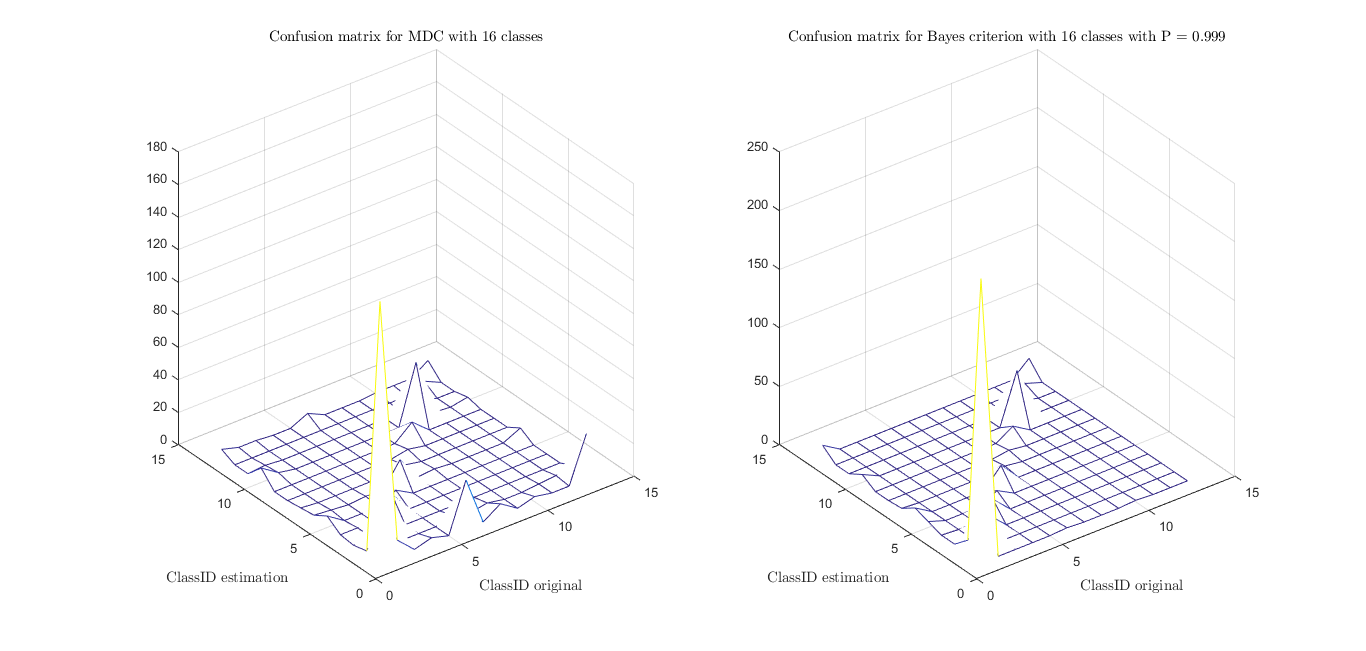
\includegraphics[scale=0.4]{pictures/confMat.png}
	\caption{Confusion matrix for 16 classes classification}\label{fig:confMat}
\end{figure}

The plot shows the improvement brought by the bayesian method with respect to MCD. Each instance in the diagonal is a correct detection, elsewhere the estimation is different from the true class. As it has been discussed above, if the percentage of the eigenvalues grows, perfomances improve.

\begin{center}
  \begin{tabular}{ | l | c | r | }
    \hline
     & Minimum Distance & Bayes approach \\ \hline
    True detection & 67.3\% & 89.6\% \\ 
    \hline
  \end{tabular}
\end{center}

\section{Clustering}
\subsection{K-means introduction}
Differentely from classification, clustering techniques is an instance of unsupervised learning. The dataset is still the same of the classification one. Now, it is considered without the known arrythmia classes column. The aim of clustering is to explore data, find some common patterns and group them into clusters with similar characteristics. The analysed clustering algorithm, called K-means, is still distance based: during the assignment, a measurement is associated to a centroid if it is closer to it than to the other ones. During the update, the centroid of the region will be the mean value of all the points associated to that region. It goes on iteratively until the convergence, or a stopping condition.

\subsection{Hard K-means 2 clusters}
The first task aims to apply hard K-means to the normalized dataset with 2 clusters starting from 2 different initial centroid positions: the classification one and random. Instead of distances, the used criterion is maximum a posteriori, where posterior probability is maximized. It starts by randomly placing k centroids in a multidimensional dimensional space, setting variance values to 1 and prior probabilities to 1/k per each cluster (initial step), then run through the dataset and find the nearest centroid per each observation (assignment step). Then, within each cluster, we recompute centroid position by averaging all points belonging to it, prior probabilities, distances per each instance and variances (update step). Algorithm converges when every point does not change from two different iterations. The complexity of the algorithm is proportional to the number of iterations times the number of clusters times the number of instances times dataset dimensions. 
In the end, performances will be assessed by computing the difference of the distance vectors and comparing the clustering with the classification obtained in the previous laboratory. 

\subparagraph{Stating from classification distances}
Initial centroid positions are the same positions found in classification problem. It has been observed that if only an iteration is computer, distance vectors are of course the same of the ones obtained with the MDC approach (with prior probabilities locked to 1/k). Results are a little bit poorer than previous case because clustering takes into account unknown features extracted from data, and it could clusters patients in a different way; while doctors are only interested in arrythmia diagnosis, so they may weight more some features than others, creating an important difference between classes and clusters.
The number of iteration has been set to 10: increasing this value, it has been seen that performances in terms of sensitivity and specificity do not change anymore. 

\subparagraph{Starting from random distances}
For random distances vectors, things change a little bit with respect to the previous case. For a small number of iterations, sensitivity and specificity appears to be very small, as it is reasonable to think about. Each time script runs, result is always different because of the different starting points.\\

Silhouette plots was done in order to show how a datum is properly assigned to a cluster: one of the two cluster appears to be more "correct" than the other one for both feature 5 and 7 (Figure \ref{fig:silhouette2cl}).\\

In order to show graphically the clusters, a PCA has been performed and data set has been reduced to 2 dimensions: the result is not that good because there is not a clear distintction among the clusters, maybe because of PCA itself. A possible technique to perform a graphical visualization is t-distributed stochastic neighbor embedding (t-SNE). 

\subsection{K-means 4 clusters}
Clustering was repeated following the same algorithm, but considering 4 clusters. Two different initial distance vectors was chosen, and again results. 
 
\lstinputlisting[caption = {Arrythmia analysis - Main}]{scripts/ArrythmiaClassification_Clustering.m}\label{lst: Arrythmia analysis - Main}
\lstinputlisting[caption = {2 Classes probabilities}]{scripts/prob2Class.m}\label{lst: 2 classes probabilities}

\begin{figure}[H]
	\centering
	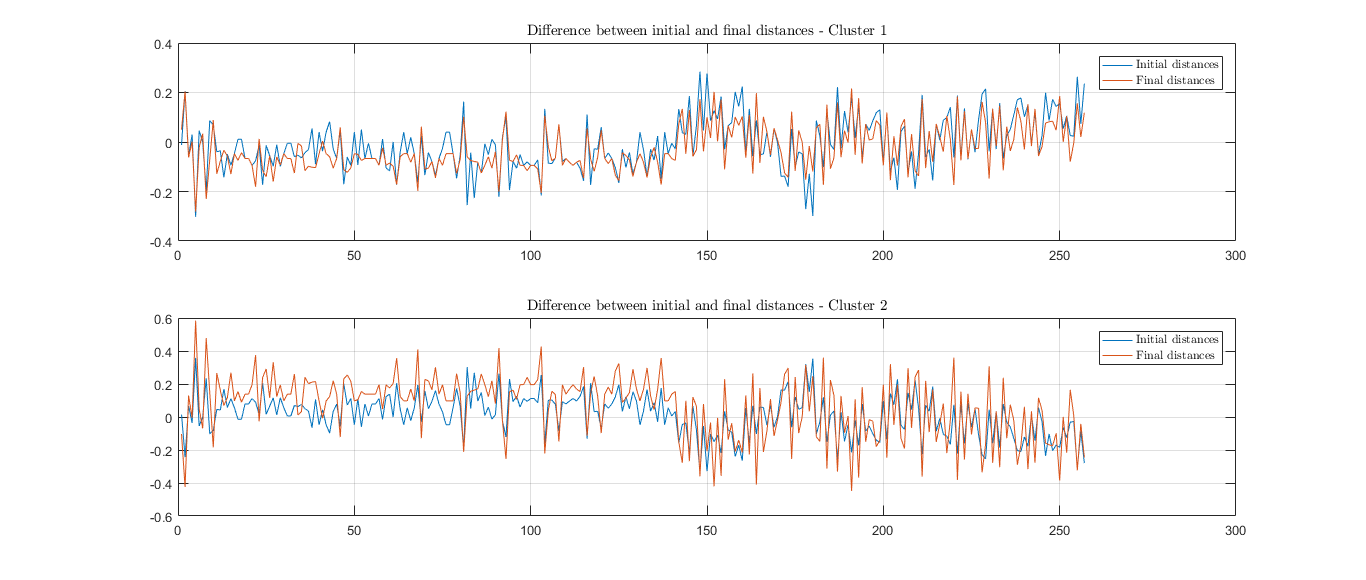
\includegraphics[width=1\textwidth]{pictures/kmeans_2clust_perf.png}
	\caption{Hard K-means - distance vectors from classification ones}\label{fig:kmeans_2clust_perf}
\end{figure}

\begin{figure}[H]
	\centering
	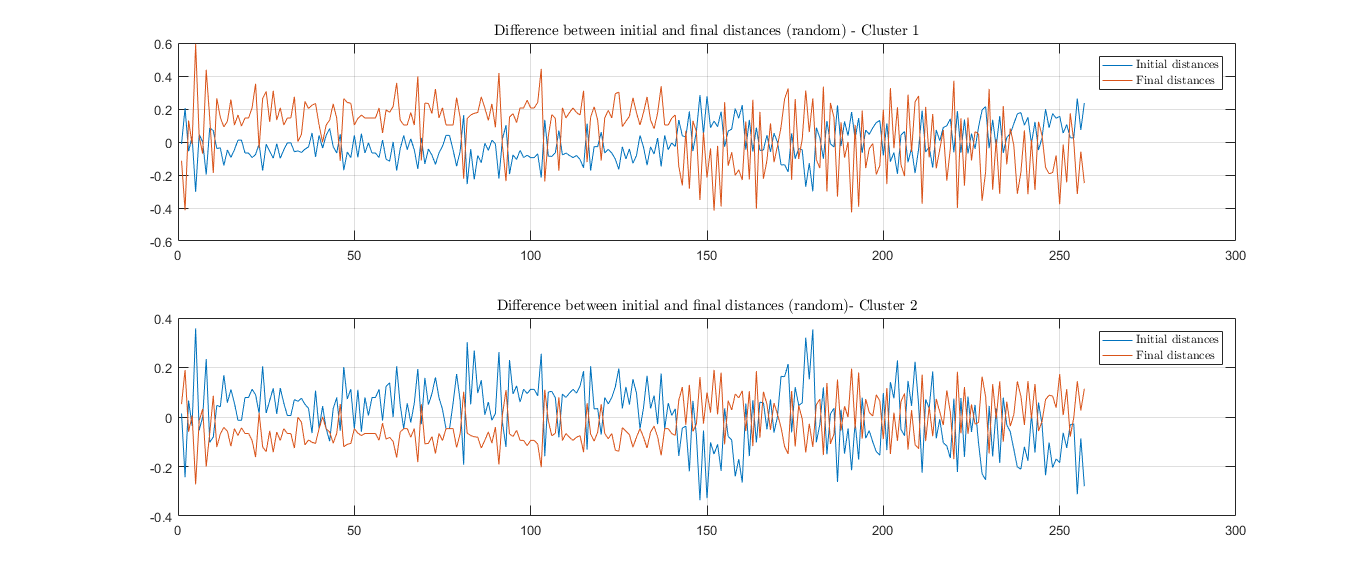
\includegraphics[width=1\textwidth]{pictures/kmeans_random_2clust.png}
	\caption{Hard K-means - distance vectors from random ones}\label{fig:kmeans_2_clust_random}
\end{figure}

\begin{figure}[H]
	\centering
	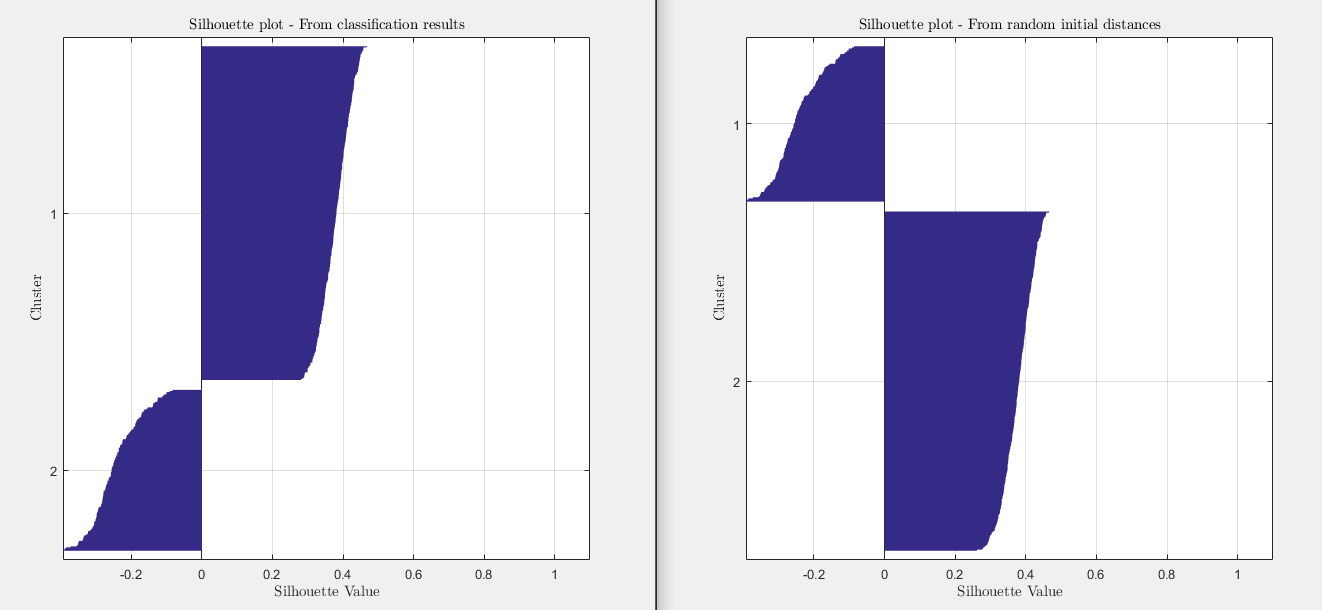
\includegraphics[width=0.85\textwidth]{pictures/silhouette2cl.png}
	\caption{Silhouette plot for 2 clusters}\label{fig:silhouette2cl}
\end{figure}

\begin{figure}[H]
	\centering
	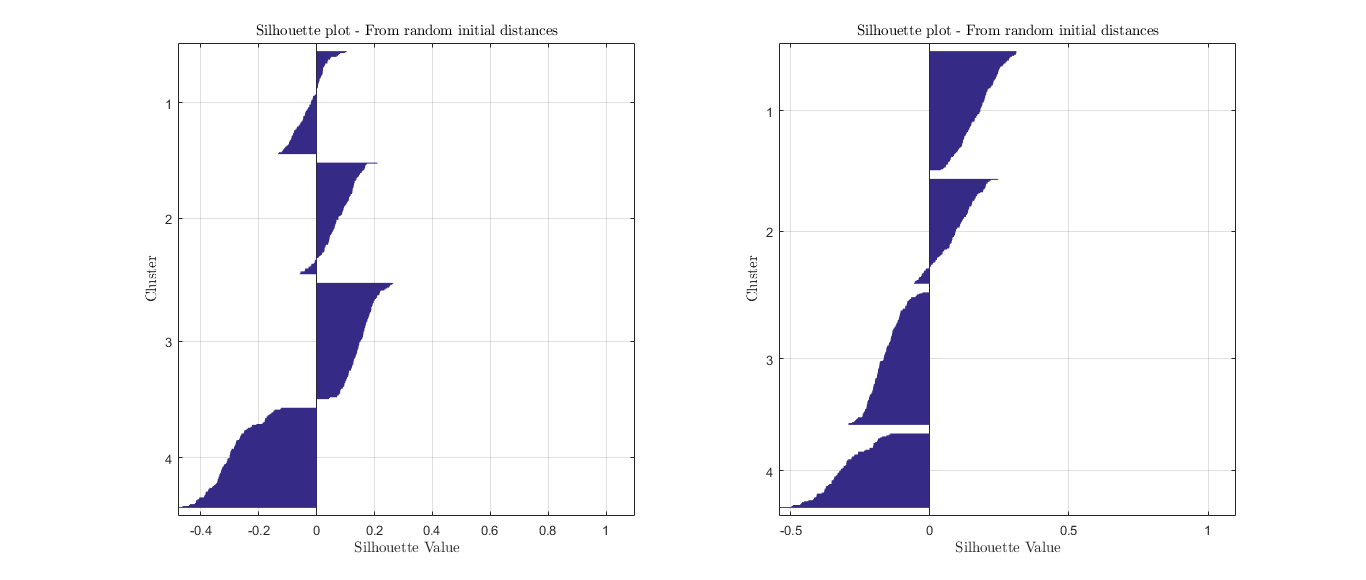
\includegraphics[width=1\textwidth]{pictures/silhouette4cl.png}
	\caption{Silhouette plot for 4 clusters}\label{fig:silhouette4cl}
\end{figure}

\newpage
\section{Hierarchical trees}
\subsection{Introduction}
The aim of this exercise deals with the application of hierarchical clustering on \href{https://archive.ics.uci.edu/ml/datasets/Chronic_Kidney_Disease}{chronic kidney disease UCI dataset}. Hierarchical clustering focuses on creation of a clusters structure. Basically, the used strategy is "agglomerative": it has a bottom up approach. It means that, initially, each observation forms a cluster; then, per each two observations, a distance is computed. The two minimum distance observations will be clustered in the same object, and so on until a unique cluster is got (root). This method has basically two main advantages: 
\begin{itemize}
	\item No need for clusters initial guess
	\item Dendrogram (a binary tree) allows to choose the suitable depth and change the number of clusters.
\end{itemize}

Distances between objects is a very crucial element of hierarchical clustering because there are a lot of criteria which can be used, and sometimes may produce very different results. Performances of different clusterings are measured by evaluating the sum of squared error: the less it is, the better is the result.\\

For this exercise, this dataset presents some non-numerical features, such that it is not possible to perform the canonical operations. For this reason, each of the nominal features has to be converted into numerical values. 

\subsection{Hierarchical clustering}
On the obtained dataset, a hierarchical clusering has been performed by using a set of MATLAB functions:
\begin{itemize}
	\item pdist: returns a vector containing the distance bewteen each two observations. A parameter is to be set in order to choose what kind of distance criterion
	\item linkage: generates the tree specifying how to measure the distances between clusters
	\item dendrogram: shows the resulting tree generated by linkage function
	\item  cluster: returns the vector containing the resulting cluster per each observation
\end{itemize}

In this analysis, pdist distance is the default one (euclidean distance). While four different linkage distance parameters was choosen: single, average, centroid and complete. For all of them, clustering results are exactly the same, with a correct detection with respect the doctors classification of 80.5\%, so there is not any difference in terms of error probability. Graph \ref{fig:dendrograms} show the different dendrograms.

\subsection{Hierarchical classification}
For hierarchical classification, was used "fitctree" function which allows binary classification decision tree for multiclass classification (see graph \ref{fig:Decision tree}). From the initial dataset, the most meaningful feature are used to split it into subranges that generate new branches of the tree, and so on until all features are analyzed. It should be convenient to perform Karhunen-Loeve decomposition in order to get some uncorrelated features, but due to some NaN entry, this is not possible. 
However, the tree gives the rules for the decision regions: in this case the correct detection probability is 82.5\%. Even if this evaluation is a little bit compromised by the presence of some "NaN" entries. \\
Click \ref{lst: Hierarchical trees} for checking the used code.

\lstinputlisting[caption = {Hierarchical trees}]{scripts/HierarchicalClustering.m}\label{lst: Hierarchical trees}

\begin{figure}[H]
	\centering
	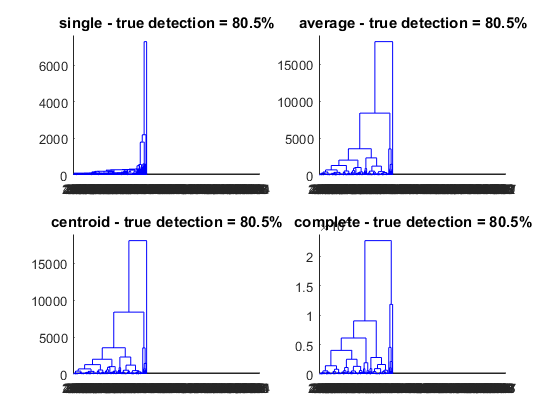
\includegraphics[width=0.8\textwidth]{pictures/dendrograms.png}
	\caption{Dendrograms}\label{fig:dendrograms}
\end{figure}

\begin{figure}[H]
	\centering
	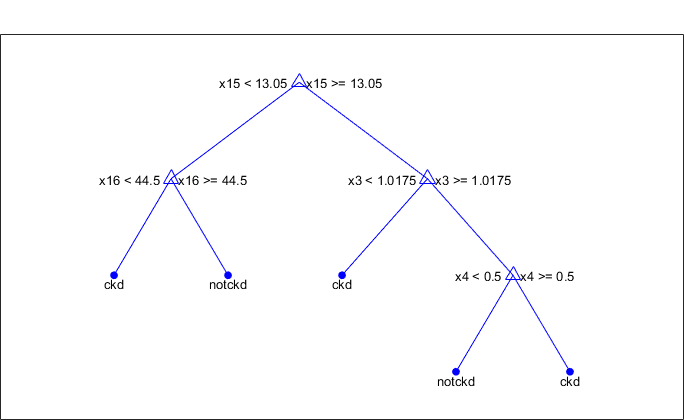
\includegraphics[width=0.8\textwidth]{pictures/decisionTree.png}
	\caption{Decision tree}\label{fig:Decision tree}
\end{figure}


\newpage
\section{Neural networks: Tensorflow}
\subsection{Introduction}
This exercise recalls the very first one: dataset is about Parkinson disease affected patients' voice. Regression is performed on the same features of the first section, but now has been used a neural network built thanks to a Google open source library called Tensorflow. The core of Tensorflow approach is divided in two parts: building and runing the computational graph.\\
Normalized data was imported thanks to the Scipy library, and all parameters have been set equal to the MATLAB case in order to compare obtained results. 








%\lstinputlisting[language=Python]{source_filename.py}
\newpage
\begin{appendix}
	\listoffigures
	\newpage
	\lstlistoflistings
\end{appendix}

\end{document}